\chapter*{Introducción}\label{chapter:introduction}
\addcontentsline{toc}{chapter}{Introducción}


% @NOTE Durante la subasta lo que se hace es que los miembros de un banco o cualquier entidad que esté participando en la subasta, aprueban o no la oferta hecha por alguien a nombre de esta organización.  Las votaciones de este tipo se realizan para confeccionar lo Comités de Mercado financiero

% @NOTE En la subasta puede pasar que algún miembro de alguna organización, transfiera su poder de decisión a otro, a la hora de aceptar una oferta

El banco \todo{@TODO qu\'e banco es? metropolitano, BPA, ...?} le ofrece pr\'estamos a entidades del estado cubano. \todo[fancyline]{@TODO poner ejemplos de entidades prestatarias} El banco  decide mediante una subasta el valor e inter\'es de cada pr\'estamo que ofrece. Durante este proceso, se confeccionan los Comit\'es de Mercado Financiero (CMF). \todo{@TODO qu\'e son los comit\'es esos?} Para elegir los miembros y el presidente de cada Comit\'e, se efect\'ua un proceso electoral en el que cualquier elector puede ceder su poder de voto a otro elector. A ese tipo de elecci\'on se le conoce como \textbf{votaci\'on representativa}.  \todo[inline]{@audit me huele a que aqu\'i va una referencia o al menos buscar bien si a eso se le llama votaci\'on representativa} 

En un sistema de votaci\'on representativa  los votos se transfieren, esto es, si una persona $A$ vota por una persona $B$ y esta, a su vez, vota por  $C$, entonces el voto de $A$ se transfiere a $C$. En el caso particular de la confecci\'on de los CMF, cada individuo puede votar por a lo sumo otra persona.

La figura \ref{fig:r-voting} ilustra un ejemplo de votación en el que $A$ votó por $B$, $B$ y $E$ votaron por $C$ y $C$ votó por $D$. $B$ obtiene solamente el voto de $A$, mientras que $C$ obtiene los votos de $A$, $B$ y $E$. $D$ recibe el voto directo de $C$ y, con este,  los votos indirectos de los restantes participantes.

\begin{figure}[h]
    \centering
    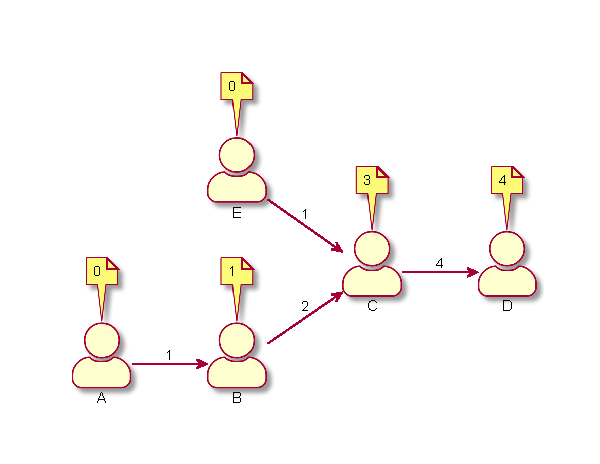
\includegraphics{Graphics/rep-voting.pdf}
    \caption{Conteo de votos en votación representativa.}
    \label{fig:r-voting}
\end{figure}

En un proceso electoral de este tipo pueden surgir ciclos de votación, como el que se muestra en la figura \ref{fig:voting-cycle}, donde el voto emitido por $D$ hacia $B$ forma un ciclo que los involucra a ambos y a $C$. En tal caso, no queda claro cu\'antos votos otorgarle a las personas involucradas en el ciclo.  Uno de los objetivos del presente trabajo es \textbf{dise\~nar e implementar una asignaci\'on justa de  votos para los electores involucrados en un ciclo de votación}. 

\begin{figure}[h]
    \centering
    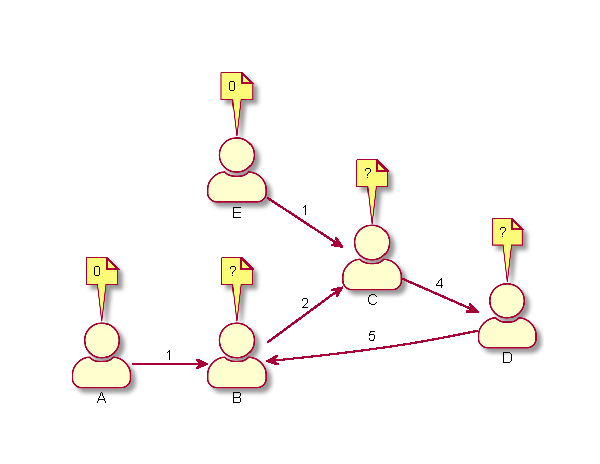
\includegraphics{Graphics/voting-cycle.pdf}
    \caption{Ciclo de votaci\'on.}
    \label{fig:voting-cycle}
\end{figure}

Para seleccionar un presidente para un CMF, se realiza una elecci\'on representativa y el que obtenga la mayor cantidad de votos es el ganador. Puede pasar que m\'as de una persona obtenga la mayor cantidad de votos.   Esto no es deseable, ya que el presidente debe ser \'unico. En este sentido, otro de los objetivos de este trabajo es \textbf{dise\~nar e implementar un mecanismo de desempate}.

% pa mantener un sistema distribuido de gouorum es necesario al menos 4 nodos % @NOTE chekea eso 

Tradicionalmente en estas elecciones, como en muchas otras, los votos son emitidos en boletas de papel y el conteo es realizado manualmente. Esto puede traer consigo ciertos problemas que causan desconfianza en el electorado, como son los votos falsos y el mal conteo de los votos.   Si no se hace una verificaci\'on rigurosa de la identidad del votante, entonces se puede emitir votos con relativa facilidad en nombre de personas que no han votado (votos falsos). Si el conteo no est\'a supervisado adecuadamente, pueden surgir errores en los resultados, ya sea por intereses personales o errores humanos.

En un sistema de votaci\'on electr\'onico se  pueden lograr diversas formas de verificaci\'on biom\'etrica, por ejemplo, mediante la huella digital o el esc\'aner ocular. Por otro lado, en estos sistemas se puede contar los votos de manera eficiente mientras se van realizando y se  puede publicar en vivo los resultados. 

Otras bondades poseen los sistemas electrónicos, como son la flexibilidad, lo fácil que pueden ser de usar y lo baratos que resultan con respecto a los sistemas tradicionales. Sin embargo, muchos de los sistemas electrónicos existentes son centralizados, esto es, dependen de que una agencia central se encargue de registrar, manejar, calcular y revisar los votos. Toda la confianza debe entonces ser depositada en esa agencia, lo cual hace vulnerable al sistema.
 
Un sistema digital descentralizado de votación no tiene ese problema. Entre las tecnologías descentralizadas más empleadas actualmente se encuentra \textit{blockchain}. \todo{@TODO explicar lo que es blockchain} 
\todo[inline]{@TODO mencionar en la explicaci\'on de blockchain que se basa en la criptograf\'ia pa que de paso menciones en la rama en la que vas a desarrollar la tesis}

% Hacerlo con \textit{blockchain} ta bueno xq resuelve la parte m\'as importante de esos problemas. 

Desde el surgimiento de Ethereum se puede implementar comportamientos complejos mediante contratos inteligentes. \todo{@TODO explicar Ethereum y contratos}   

No es deseable que el proceso electoral en el CMF se realice en una red p\'ublica, ya que es un proceso que s\'olo concierne a las partes involucradas. Por otro lado, desplegar un contrato inteligente en Ethereum puede costar miles de d\'olares (\cite{eth-deploy}). Estos dos factores hacen que no sea factible realizar la implementaci\'on de este trabajo sobre la red p\'ublica de Ethereum. 

GoQuorum es una implementaci\'on de Ethereum capaz de crear redes privadas y con mecanismos de autorizaci\'on. En GoQuorum tambi\'en se puede personalizar el costo del despliegue de los contratos inteligentes, incluso, puede hacerse nulo. Por todo lo dicho anteriormente, GoQuorum es una buena opci\'on en la que implementar el sistema de votaci\'on representativa del CMF.


Existen implementaciones de sistemas de votaci\'on en otras \textit{blockchain} (\cite{agora}) y tambi\'en en Ethereum (\cite{ovn} y \cite{borda_count}), pero no se conoce ninguna implementaci\'on de un sistema de voto representativo en GoQuorum.

\todo[inline]{@TODO decir que el Instituto de Criptograf\'ia implement\'o un sistema de votaci\'on en hyperledger fabric pero tampoco nos sirve. ?`C\'omo cito eso?}


Con el presente trabajo de diploma  se pretende dise\~nar e implementar un sistema de votaci\'on representativa en GoQuorum. El sistema debe ser capaz de realizar elecciones para un CMF, asignando un valor justo de votos para los electores involucrados en un ciclo de votaci\'on y determinando un ganador, incluso cuando hay empate en el primer lugar. El sistema debe ser lo m\'as gen\'erico posible, de forma tal que sea factible su uso m\'as all\'a del entorno bancario.


\todo[inline]{@audit no s\'e si aqu\'i poner algunos requisitos de \cite{wang2017review} que pensamos que el sistema debe cumplir o simplemente citar ese art\'iculo y decir que el sistema debe ser implementado de forma tal que cumpla la mayor cantidad de requisitos posibles}


% estudiar, disenyar y modelar, implementar y evaluar resultados

% @TODO decir d q' va cada capi'tulo

% @NOTE habla en tiempo presente, 3ra persona del singular, e.g. "el autor ha desarrollado", "el autor ha realizado", etc.